\begin{figure*}[htbp]
    \centering%
    \setlength{\tabcolsep}{0.002\textwidth}%
    \renewcommand{\arraystretch}{1}%
    \footnotesize%
    \begin{tabular}{ccccccc}
        Initial asset & \multicolumn{6}{c}{
            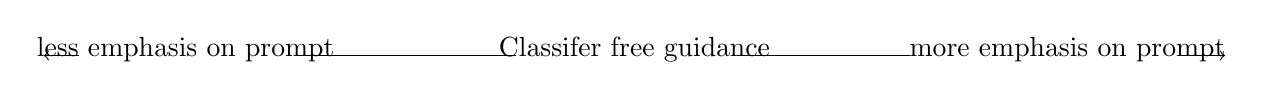
\begin{tikzpicture}
                \draw[<-] (0,0) -- (0.45,0);
                \draw[-] (3.2,0) -- (6.0,0);
                \draw[-] (8.8,0) -- (11,0);
                \draw[->] (14.4,0) -- (15,0);
                \node[above] at (1.8,-0.2) {less emphasis on prompt};
                \node[above] at (7.5,-0.2) {Classifer free guidance};
                \node[above] at (13,-0.2) {more emphasis on prompt};
            \end{tikzpicture}
        }\\[-4pt]%
        & 4.0 & \textbf{7.5} & 11.0 & 14.5 & 18.0 & 21.5\\%
        \includegraphics[height=0.14\linewidth]{figures/secondary_hparams/initial/0001.png}&%
        \includegraphics[height=0.14\linewidth]{figures/secondary_hparams/guidance_4.0_001.jpg}&%
        \includegraphics[height=0.14\linewidth]{figures/secondary_hparams/guidance_7.5_001.jpg}&%
        \includegraphics[height=0.14\linewidth]{figures/secondary_hparams/guidance_11.0_001.jpg}&%
        \includegraphics[height=0.14\linewidth]{figures/secondary_hparams/guidance_14.5_001.jpg}&%
        \includegraphics[height=0.14\linewidth]{figures/secondary_hparams/guidance_18.0_001.jpg}&%
        \includegraphics[height=0.14\linewidth]{figures/secondary_hparams/guidance_21.5_001.jpg}
    \end{tabular}%
    \caption{Controlling the magnitude of detail enhancements using classifier free guidance.
    The scaling factor allows the user to apply more conservative changes and stay closer to the input or obtain more pronounced changes, as desired.}
    \label{fig:hparams_usercontrol}
\end{figure*}
